%% main.tex — UAV-Based Neural Reconstruction of Dong Drum Towers
%% Target: IEEE TVCG / TVC
%% Author: Jiaxing Tao (Kaili College)
%%==================================================================
\documentclass[journal,onecolumn,11pt]{IEEEtran}

%% ---- Packages ----
\usepackage[utf8]{inputenc}
\usepackage[T1]{fontenc}
\usepackage{amsmath,amssymb,amsfonts}
\usepackage{graphicx}
\usepackage{booktabs}
\usepackage{multirow}
\usepackage{multicol}
\usepackage{url}
\usepackage{hyperref}
\usepackage{xcolor}
\usepackage{algorithm}
\usepackage{algorithmic}
\usepackage{subcaption}
\usepackage{enumitem}
\usepackage{makecell}
\usepackage{longtable}
\usepackage{booktabs}
\usepackage{array}
\usepackage{multirow}
\usepackage{calc}


\hypersetup{
    colorlinks=true,
    linkcolor=blue,
    citecolor=blue,
    urlcolor=blue,
    pdftitle={UAV-Based Neural Reconstruction of Dong Drum Towers: A Multi-Case Benchmark for Conservation-Oriented Method Selection},
    pdfauthor={Jiaxing Tao},
    pdfkeywords={Dong drum tower, neural reconstruction, UAV photogrammetry, NeRF, 3D Gaussian Splatting, 2D Gaussian Splatting, Instant-NGP, heritage documentation, benchmark}
}

%% ---- Custom commands ----
\newcommand{\todo}[1]{\textcolor{red}{\textbf{[TODO: #1]}}}
\newcommand{\note}[1]{\textcolor{orange}{\textit{[#1]}}}
\newcommand{\ours}{DrumTower}

%% ---- Graphics path ----
\graphicspath{{figures/}{figures/results/}}

\begin{document}

\title{UAV-Based Neural Reconstruction of Dong Drum Towers: A Multi-Case Benchmark for Conservation-Oriented Method Selection}

\author{
    \IEEEauthorblockN{Jiaxing Tao}
    \IEEEauthorblockA{
        Department of Computer Science and Technology\\
        Kaili College, Guizhou, China\\
        Email: \url{1793690143@qq.com}
    }
}

\maketitle

%% ---- Abstract & Keywords ----
%% sections/abstract.tex

\begin{abstract}
3D Gaussian Splatting (3DGS) has emerged as a transformative approach for
real-time radiance field rendering, combining the representational power of
explicit 3D primitives with differentiable rasterization.
Since the seminal work of Kerbl et~al.\ (2023), the field has experienced
explosive growth, with over \todo{N} papers published within two years.
However, this rapid expansion has led to a fragmented landscape where
contributions are difficult to compare and contextualize.

In this survey, we present a comprehensive taxonomy of 3DGS research,
organized along three orthogonal axes: \textbf{(1)~Task Domain}
(reconstruction, dynamic/4D, editing, generation, compression),
\textbf{(2)~Module Focus} (representation, optimization, rendering,
initialization, densification), and \textbf{(3)~Technique}
(anchoring, compression, anti-aliasing, regularization, level-of-detail,
feature augmentation).
We further introduce the \textbf{Drum Tower Dataset}, a new real-world
benchmark featuring Chinese Dong minority architecture with intricate
wooden structures and multi-scale geometry.
Our extensive experiments evaluate \todo{12} representative methods across
\todo{5} datasets, providing detailed analysis of quality-speed trade-offs,
memory consumption, and geometric accuracy.
Finally, we identify open challenges and promising future directions,
including scene-level understanding, physics-aware representations,
and edge-device deployment.

The project page and benchmark code are available at
\url{https://github.com/autumn119/3DGS-Survey-Taxonomy-Benchmark}.
\end{abstract}

\begin{IEEEkeywords}
3D Gaussian Splatting, Novel View Synthesis, Neural Rendering,
Radiance Fields, Survey, Benchmark, Taxonomy
\end{IEEEkeywords}


%% ---- Body ----
%% sections/abstract.tex

\begin{abstract}
3D Gaussian Splatting (3DGS) has emerged as a transformative approach for
real-time radiance field rendering, combining the representational power of
explicit 3D primitives with differentiable rasterization.
Since the seminal work of Kerbl et~al.\ (2023), the field has experienced
explosive growth, with over \todo{N} papers published within two years.
However, this rapid expansion has led to a fragmented landscape where
contributions are difficult to compare and contextualize.

In this survey, we present a comprehensive taxonomy of 3DGS research,
organized along three orthogonal axes: \textbf{(1)~Task Domain}
(reconstruction, dynamic/4D, editing, generation, compression),
\textbf{(2)~Module Focus} (representation, optimization, rendering,
initialization, densification), and \textbf{(3)~Technique}
(anchoring, compression, anti-aliasing, regularization, level-of-detail,
feature augmentation).
We further introduce the \textbf{Drum Tower Dataset}, a new real-world
benchmark featuring Chinese Dong minority architecture with intricate
wooden structures and multi-scale geometry.
Our extensive experiments evaluate \todo{12} representative methods across
\todo{5} datasets, providing detailed analysis of quality-speed trade-offs,
memory consumption, and geometric accuracy.
Finally, we identify open challenges and promising future directions,
including scene-level understanding, physics-aware representations,
and edge-device deployment.

The project page and benchmark code are available at
\url{https://github.com/autumn119/3DGS-Survey-Taxonomy-Benchmark}.
\end{abstract}

\begin{IEEEkeywords}
3D Gaussian Splatting, Novel View Synthesis, Neural Rendering,
Radiance Fields, Survey, Benchmark, Taxonomy
\end{IEEEkeywords}

%% sections/introduction.tex
\section{Introduction}\label{introduction}

Dong drum towers are among the most representative public timber
structures in traditional Dong villages in Southwest China, particularly
in Guizhou, Hunan, and Guangxi. As architectural landmarks and communal
infrastructures, they embody the regional identity, social organization,
construction knowledge, ritual life, and collective memory of Dong
communities. Typically constructed from Chinese fir or other locally
treated timber, drum towers are assembled through mortise-and-tenon
joints without the use of nails or metal fasteners, forming compact,
durable, and highly hierarchical wooden structures. Their elevated
columns, interlocking beams, layered eaves, roof-crown systems, and
tiered supporting frameworks reflect the craftsmanship and structural
ingenuity of Dong master carpenters. Historically, drum towers served as
central public spaces for village assemblies, covenant making, warning
against external threats, festive gatherings, musical performance, and
intergenerational cultural transmission. Their architectural form is
therefore not merely a physical construction, but a material carrier of
community practice, craft knowledge, spatial order, and intangible
cultural heritage.

Previous studies have examined Dong drum towers from multiple
perspectives, including construction techniques, structural typologies,
regional distribution, roof-crown systems, bracket components, and
master-carpenter knowledge, thereby establishing a fundamental
architectural understanding of this distinctive timber heritage type
[1--5]. At the settlement scale, further research has shown that
drum towers are closely embedded in the spatial organization, cultural
transformation, and design preferences of Dong villages [6,7]. These
studies demonstrate that drum towers should be understood as both
technical timber structures and socio-cultural infrastructures. As shown
in Fig. 1, their morphological characteristics, including eave
hierarchy, roof type, plan configuration, tower height, and crown form,
reveal substantial diversity across different villages and construction
traditions.

\begin{figure}[htbp]
    \centering
    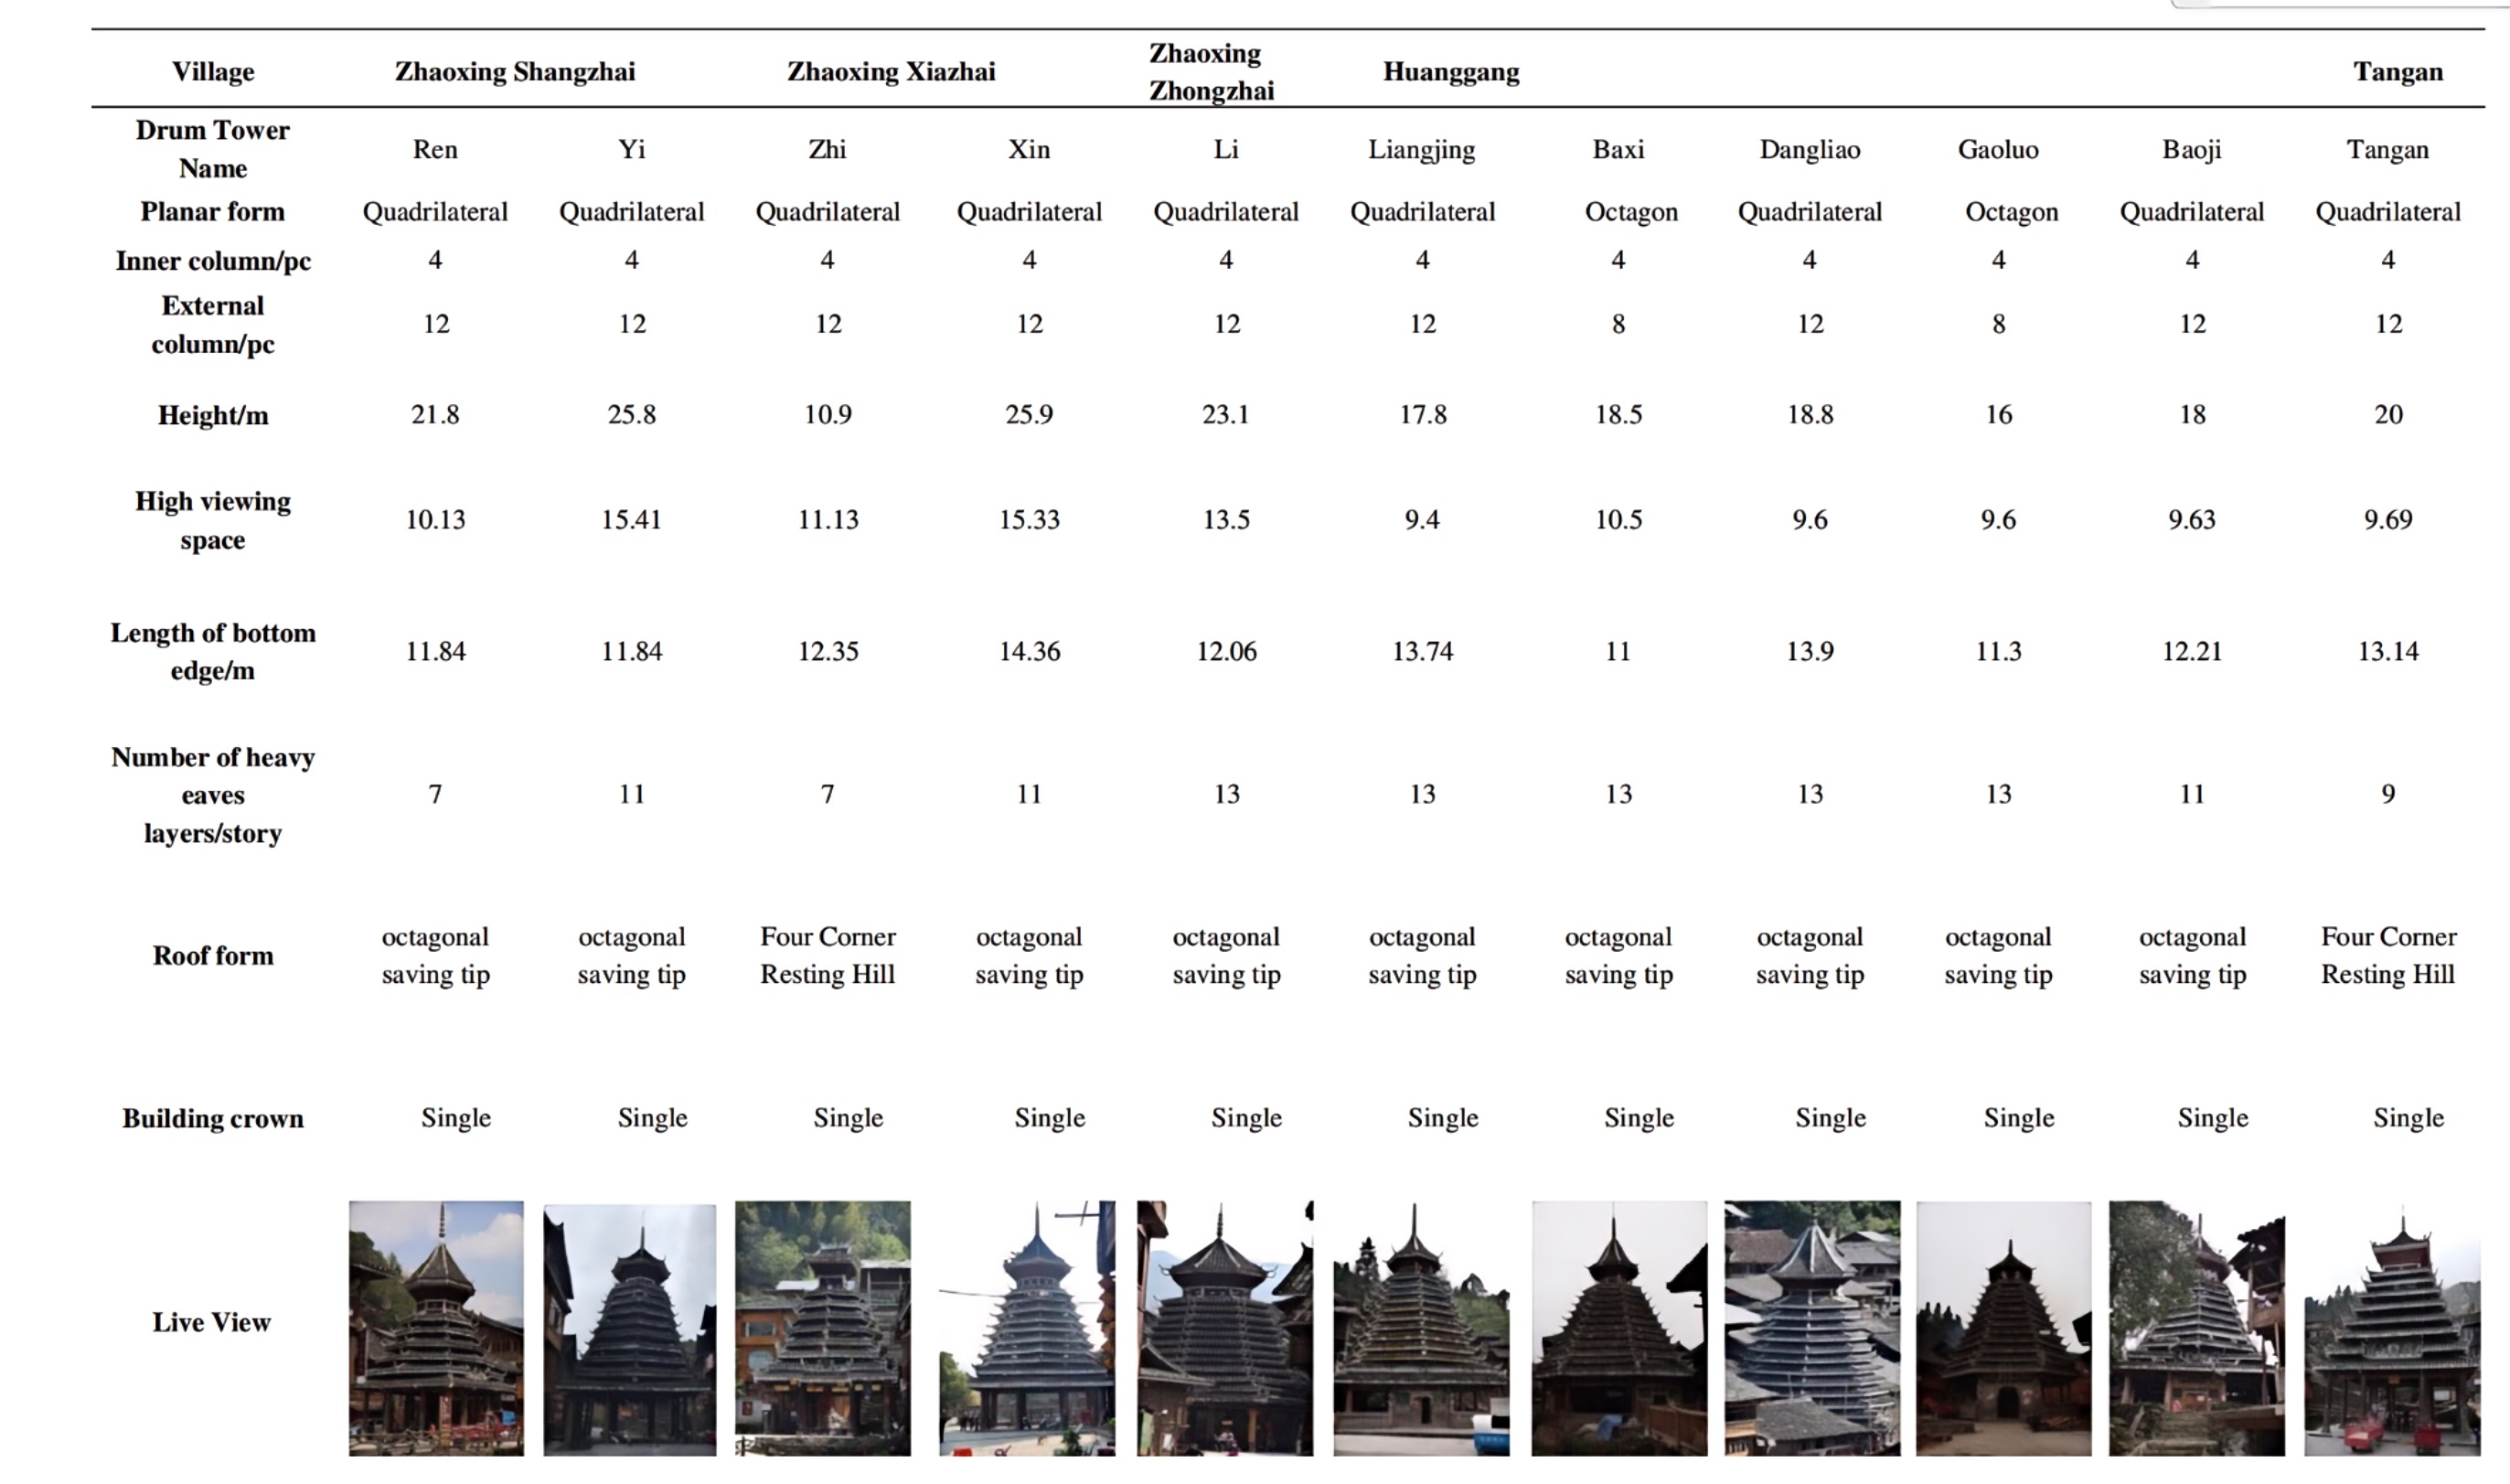
\includegraphics[width=\linewidth]{figures/media/image1}
    \label{fig:pandoc_1}
\end{figure}


\begin{figure}[htbp]
    \centering
    \includegraphics[width=\linewidth]{figures/media/image2}
    \label{fig:pandoc_2}
\end{figure}


\textbf{Fig. 1. Morphological characteristics and spatial forms of
representative Dong drum towers[8].}

Recent scholarship has extended Dong drum tower research from
architectural description to digital heritage, acoustic simulation,
mathematical metamodeling, UAV-based reconstruction, and intelligent
heritage building information modeling. Mao et al. demonstrated that the
spatial form of Dong drum towers is closely associated with sound-field
characteristics and ceremonial use [9]. Deng et al. proposed
mathematical metamodeling for automated simulation of Dong drum tower
architectural heritage, highlighting the possibility of computational
representation of traditional timber structures [10]. Huang et al.
developed a digital preservation workflow for endangered Dong drum
towers by integrating field investigation, UAV documentation, BIM, and
3D reconstruction [11]. Deng et al. further introduced an
intelligent HBIM framework that combines machine vision and
architectural expertise for traditional timber heritage, validating its
applicability using Dong drum tower data [12]. Related studies on
Dong soundscapes and traditional village morphology also indicate that
Dong architectural heritage should be understood as a coupled system of
built form, spatial organization, acoustic experience, and community
practice [13--15].

From the perspective of heritage science, the documentation of Dong
drum towers requires more than geometric recording or visual
reproduction. International heritage frameworks have emphasized the
protection of intangible cultural practices, authenticity, and wooden
built heritage [16--18]. For timber architecture in particular,
conservation-oriented documentation must support the understanding of
material condition, structural configuration, component relationships,
construction logic, and long-term maintenance needs [19]. Digital
documentation technologies have therefore become increasingly important
in architectural heritage conservation. HBIM has been widely adopted to
connect geometric documentation, semantic information, conservation
records, and heritage management workflows [10--24]. In parallel,
photogrammetry, 3D scanning, and image-based recording techniques have
provided robust technical foundations for capturing complex heritage
morphology [25--27]. However, for highly layered timber structures
such as Dong drum towers, the central challenge is not only whether a
digital model can be generated, but whether conservation-relevant
components can be faithfully recovered, interpreted, and used for
downstream heritage tasks.

%% sections/Research_Background.tex
\section{Related Work}\label{sec:research_background}

\subsection{\textbf{2. Literature Background and
Conservation-Oriented Problem
Definition}}\label{literature-background-and-conservation-oriented-problem-definition}

Existing research has made important progress in the digital
documentation and conservation of Dong drum towers. Previous studies
have examined their architectural typologies, roof-crown forms,
construction techniques, structural components, master-carpenter
knowledge, acoustic characteristics, mathematical modeling, UAV-based
recording, BIM reconstruction, and HBIM-oriented intelligent modeling.
These studies have provided valuable foundations for understanding Dong
drum towers as complex timber heritage systems and have demonstrated the
feasibility of using digital technologies to record, visualize, and
interpret their architectural characteristics. However, much of the
existing work has focused on documentation workflows, geometric
modeling, digital representation, or heritage information management.
Less attention has been paid to how different neural reconstruction
methods perform under comparable empirical conditions and how their
outputs can be interpreted in relation to conservation-oriented
documentation needs.

Neural reconstruction methods are relevant to Dong drum tower
documentation because these structures present challenges that are
difficult to address through conventional image-based modeling alone.
Their multi-layered eaves, dense timber frameworks, repeated roof
modules, roof-crown details, and shadowed interior spaces require
methods that can handle complex appearance, partial occlusion, viewpoint
variation, and fine architectural details. NeRF-based methods provide a
mature baseline for view synthesis through continuous radiance-field
representation. INGP improves practicality by reducing training cost
through multiresolution hash encoding. 3DGS offers efficient explicit
scene representation and real-time rendering potential, making it
suitable for visually complex heritage scenes. 2DGS, although not
primarily optimized for image-level metrics in the present study,
remains relevant because of its surface-oriented formulation and
potential value for future geometry-focused evaluation. These
complementary characteristics justify a controlled comparison of NeRF,
2DGS, 3DGS, and INGP for Dong drum tower reconstruction and provide the
basis for the following discussion of conservation-relevant components
and related neural reconstruction methods.

\subsection{2.1 Conservation-Relevant Architectural Components of Dong
Drum
Towers}\label{conservation-relevant-architectural-components-of-dong-drum-towers}

For Dong drum towers, conservation-oriented documentation should focus
on architectural components that carry structural, morphological, and
cultural significance. The most critical elements include layered eaves,
roof-crown systems, columns and beams, bracket-like supporting members,
mortise-and-tenon joint areas, enclosure components, base structures,
and shadowed inner timber spaces. These components should not be
understood merely as visual features. Together, they encode the
construction logic, craft knowledge, spatial hierarchy, morphological
identity, and maintenance history of the tower.

Layered eaves are among the most visually distinctive and
conservation-relevant features of Dong drum towers. They reflect the
vertical hierarchy of the structure and the carpentry logic used to
organize repeated roof layers. However, their dense arrangement can
cause self-occlusion, repeated-texture ambiguity, and shadow
accumulation during image-based reconstruction. Roof-crown systems are
also important because they function as symbolic and morphological
markers of the tower, yet they are often small, elevated, and difficult
to capture with sufficient detail from ground-based or limited UAV
viewpoints. Timber columns, interlocking beams, bracket-like supports,
and mortise-and-tenon joint areas are essential for understanding the
structural configuration and traditional construction techniques, but
they are frequently affected by low illumination, dense wooden
intersections, and limited camera visibility.

The lower base, enclosure elements, inner timber spaces, and areas
beneath multi-layered eaves are also important for restoration survey
and periodic monitoring because they may contain traces of deformation,
material aging, moisture effects, or later repair interventions. These
areas are usually more difficult to reconstruct than exposed exterior
surfaces because of shadow, narrow viewing angles, and partial
occlusion. Therefore, a conservation-oriented evaluation of neural
reconstruction methods should not rely solely on global visual metrics.
It should also consider whether the reconstructed outputs preserve the
readability of critical architectural components and whether the results
can support practical tasks such as visual documentation, HBIM
preparation, restoration planning, digital exhibition, and long-term
monitoring.

These conservation-relevant components define the main technical
challenges for digital reconstruction. Classical registration and
model-fitting methods, such as ICP and RANSAC, provide essential support
for 3D alignment and geometric robustness, but they do not directly
address the view-synthesis and rendering challenges posed by complex
heritage scenes [28,29]. Existing-building BIM reconstruction and
large-scale 3D modeling studies have shown that complex heritage
environments often require the integration of point-cloud processing,
semantic enrichment, and object-based interpretation [30--32].
Knowledge-based HBIM enrichment and mesh-based information modeling
further indicate that high-quality reconstruction is not only a visual
task, but also a prerequisite for semantic representation and downstream
conservation use [33,34]. For Dong drum towers, these challenges are
amplified by multi-layered eaves, repeated roof geometries, dense timber
components, roof-crown details, and heavily shaded spaces beneath the
eaves.

\subsection{2.2 Related Work on Neural Reconstruction and Heritage
Documentation}\label{related-work-on-neural-reconstruction-and-heritage-documentation}

Recent advances in neural rendering have opened new possibilities for
the digital reconstruction of complex heritage scenes. Local Light Field
Fusion provided an early practical framework for view synthesis with
prescribed sampling strategies [35]. Neural Radiance Fields
demonstrated that scene geometry and appearance can be jointly encoded
as a continuous radiance field for high-quality novel-view synthesis
[36]. Mip-NeRF and Mip-NeRF 360 further improved anti-aliasing and
unbounded-scene rendering, making neural scene representation more
robust in real-world environments [37,38]. Instant-NGP greatly
reduced training cost through multiresolution hash encoding, improving
the practicality of neural rendering workflows [39]. More recently,
3D Gaussian Splatting achieved real-time radiance-field rendering with
strong visual fidelity [40], while 2D Gaussian Splatting emphasized
a more geometrically oriented surface representation [41].
Extensions such as GS-SLAM and deformable 3D Gaussians have further
demonstrated the broader applicability of Gaussian-based representations
to dense SLAM and dynamic-scene reconstruction [42,43].

In image-based rendering tasks, PSNR, SSIM, and LPIPS are widely used to
measure pixel-level fidelity, structural similarity, and perceptual
similarity, respectively [44,45]. These metrics provide a useful
basis for comparing rendered views with reference images, but they do
not fully capture the conservation value of reconstructed outputs. For
architectural heritage, especially complex timber structures,
reconstruction quality must also be interpreted in relation to component
readability, structural continuity, and downstream documentation tasks.
Research on 3D point clouds has similarly highlighted the importance of
geometry-aware interpretation and downstream spatial understanding
[46].

Despite these advances, the applicability of neural reconstruction
methods to complex timber heritage remains insufficiently examined. Most
existing studies on Dong drum towers have focused on sound-field
simulation, mathematical modeling, UAV-based documentation, or
HBIM-oriented modeling, rather than controlled cross-method evaluation
under the same empirical heritage dataset [9--12]. As a result, it
remains unclear how NeRF-, Gaussian-, and hash-encoding-based methods
behave when processing multi-eave timber structures with repeated
components, occluded spaces, and strong illumination variation. More
importantly, it remains unclear how quantitative rendering metrics,
computational efficiency, and architectural-component readability should
be jointly interpreted for practical method selection in digital
heritage workflows.

To move beyond visual demonstration toward conservation-oriented
evaluation, this study addresses three heritage-science-oriented
research questions. First, which neural reconstruction method most
reliably preserves conservation-relevant architectural components of
Dong drum towers, including layered eaves, roof-crown systems, timber
frameworks, and shadowed internal spaces? Second, how do different
neural scene representations---NeRF-based, Gaussian-based, and
hash-encoding-based---perform across heterogeneous drum tower scenes
acquired under comparable UAV imaging conditions? Third, how can
rendering fidelity, computational efficiency, and architectural-view
readability be integrated to guide task-oriented method selection for
digital documentation, rapid field reconstruction, HBIM preparation,
digital exhibition, and periodic monitoring?

To answer these questions, this study constructs a multi-case empirical
corpus using UAV images of four representative Dong drum towers: Chaoli,
Congjiang, Zeli, and Zengchong. Four neural rendering and reconstruction
methods---NeRF, 2DGS, 3DGS, and INGP---are implemented and compared
under a controlled experimental workflow based on consistent scene data,
SfM-based camera pose estimation, image screening, and train/test
splitting where applicable. Rendering quality is evaluated using PSNR,
SSIM, and LPIPS, while computational practicality is assessed through
training time and rendering speed. In addition, representative
architectural views, including the base, enclosure, main body, tower
tip, and panoramic view, are analyzed to connect metric-based evaluation
with conservation-oriented interpretation.

The main contributions of this study are fourfold. First, it establishes
a UAV-based multi-case empirical corpus for representative Dong drum
towers, providing a comparative basis for neural reconstruction research
in complex timber heritage contexts. Second, it presents a controlled
evaluation of NeRF, 2DGS, 3DGS, and INGP using consistent scene data,
camera poses, and quantitative rendering metrics. Third, it combines
PSNR, SSIM, LPIPS, training efficiency, rendering speed, and
architectural-view analysis to assess method performance from both
computational and heritage-documentation perspectives. Fourth, it
proposes a conservation-oriented interpretation framework that
translates algorithmic results into task-aware method-selection guidance
for digital visualization, rapid reconstruction, HBIM-oriented modeling,
restoration survey, and long-term monitoring of timber heritage.

Overall, this study shifts the digital reconstruction of Dong drum
towers from isolated visual demonstration toward a task-aware evaluation
framework for heritage conservation. By linking neural rendering
performance with the documentation needs of complex timber heritage, the
study provides practical evidence for selecting appropriate
reconstruction methods in conservation-oriented workflows and
contributes to the broader application of neural reconstruction
technologies in heritage science.


%% sections/study_objects.tex
\section{An in-depth study of the various features of the Drum Tower}
\label{sec:study_objects}

\subsubsection{\texorpdfstring{\textbf{\hl{3 Study
Objects}}}{3 Study Objects}}\label{study-objects}

\hl{The four selected cases---Chaoli, Congjiang, Zeli, and
Zengchong---provide a representative empirical basis for method
comparison. The external forms and structural characteristics of the
four drum towers are shown in Fig.5. This selection strategy emphasizes
heterogeneity in reconstruction difficulty, covering variations in roof
hierarchy, timber density, shadowed spaces, viewpoint continuity, and
village surroundings.}

\includegraphics[width=6.6875in,height=4.41181in]{figures/media/image7.png}

\textbf{\hl{Fig. 5. Four Dong drum tower cases.}}

\hl{As shown in Table 2, Congjiang Drum Tower has a relatively clear
external geometry, but still presents challenges in handling repetitive
timber textures and preserving local details. Zeli Drum Tower is
characterized by a distinctly layered roof structure, making it suitable
for evaluating the ability of different methods to reconstruct repeated
eave patterns and subtle depth relationships between roof tiers. Chaoli
Drum Tower represents a more complex acquisition scenario, with poor
viewpoint continuity and unstable test-view construction conditions,
which directly affect view synthesis quality and cross-method
comparability. Zengchong Drum Tower contains dense multi-layered eave
geometry and rich timber-component details, posing substantial
challenges for eva.}

\begin{longtable}[]{@{}
  >{\centering\arraybackslash}p{(\linewidth - 8\tabcolsep) * \real{0.0654}}
  >{\centering\arraybackslash}p{(\linewidth - 8\tabcolsep) * \real{0.1289}}
  >{\centering\arraybackslash}p{(\linewidth - 8\tabcolsep) * \real{0.2499}}
  >{\centering\arraybackslash}p{(\linewidth - 8\tabcolsep) * \real{0.3237}}
  >{\centering\arraybackslash}p{(\linewidth - 8\tabcolsep) * \real{0.2321}}@{}}
\caption{\textbf{\hl{Table 2. Overview of the four Dong drum tower cases
and their main reconstruction challenges}}}\tabularnewline
\toprule\noalign{}
\begin{minipage}[b]{\linewidth}\centering
\textbf{\hl{Case ID}}
\end{minipage} & \begin{minipage}[b]{\linewidth}\centering
\textbf{\hl{Scene}}
\end{minipage} & \begin{minipage}[b]{\linewidth}\centering
\textbf{\hl{Architectural characteristics}}
\end{minipage} & \begin{minipage}[b]{\linewidth}\centering
\textbf{\hl{Main reconstruction challenges}}
\end{minipage} & \begin{minipage}[b]{\linewidth}\centering
\textbf{\hl{Relevance to comparative evaluation}}
\end{minipage} \\
\midrule\noalign{}
\endfirsthead
\toprule\noalign{}
\begin{minipage}[b]{\linewidth}\centering
\textbf{\hl{Case ID}}
\end{minipage} & \begin{minipage}[b]{\linewidth}\centering
\textbf{\hl{Scene}}
\end{minipage} & \begin{minipage}[b]{\linewidth}\centering
\textbf{\hl{Architectural characteristics}}
\end{minipage} & \begin{minipage}[b]{\linewidth}\centering
\textbf{\hl{Main reconstruction challenges}}
\end{minipage} & \begin{minipage}[b]{\linewidth}\centering
\textbf{\hl{Relevance to comparative evaluation}}
\end{minipage} \\
\midrule\noalign{}
\endhead
\bottomrule\noalign{}
\endlastfoot
\hl{DDT-01} & \hl{Chaoli Drum Tower} & \hl{Multi-layered timber tower
with complex roof hierarchy} & \hl{Large viewpoint discontinuities;
unstable test-view construction; shadowed eave regions} & \hl{Testing
robustness under difficult acquisition conditions} \\
\hl{DDT-02} & \hl{Congjiang Drum Tower} & \hl{Distinct external geometry
with relatively regular overall form} & \hl{Repetitive timber textures;
local detail preservation} & \hl{Comparing rendering fidelity and
texture reconstruction} \\
\hl{DDT-03} & \hl{Zeli Drum Tower} & \hl{Strongly layered roof structure
with repeated eave patterns} & \hl{Repeated roof geometry; depth
ambiguity between eave layers} & \hl{Evaluating structural consistency
in complex roof regions} \\
\hl{DDT-04} & \hl{Zengchong Drum Tower} & \hl{Dense multi-eave geometry
with rich timber details} & \hl{Dense components; high-frequency detail
preservation; shadowed regions} & \hl{Testing detail reconstruction and
rendering robustness} \\
\end{longtable}

\subsection{\texorpdfstring{\hl{3.1 UAV Data Acquisition and Image
Corpus
Construction}}{3.1 UAV Data Acquisition and Image Corpus Construction}}\label{uav-data-acquisition-and-image-corpus-construction}

UAV images were acquired using a DJI Air 2S platform equipped with its
integrated camera sensor. The acquisition strategy was designed to
record the external morphology of the selected Dong drum towers as
completely as possible, including roof-crown structures, layered eaves,
timber façades, and immediate spatial surroundings. To balance global
coverage and local detail recording, the field campaign combined
sequential video recording for overall scene capture with still-image
acquisition for local observations. Multi-height and multi-angle views
were collected where site conditions allowed.

The acquisition parameters and image corpus information are summarized
in Table 3. In this study, overlap refers to the approximate average
overlap between adjacent UAV images during acquisition. Because the
source records provide only average overlap values rather than separate
forward and side overlap, the values are reported as nominal overlap
indicators. They are used to describe acquisition density and image
redundancy, not as independently measured forward- and side-overlap
parameters.

For Congjiang and Zengchong, twenty ground control points were measured
using Qianxun SR6 Plus differential GPS, with reported positioning error
below 1 cm. For Chaoli and Zeli, no GCP/RTK information is available;
therefore, scale reliability in these scenes should be interpreted with
caution and, where possible, checked against measurable architectural
dimensions such as total height, base width, column spacing, or eave
width. Weather and lighting conditions were not systematically recorded
during the field campaign; this limitation is acknowledged in the later
discussion.

All images were standardized to a resolution of 1920 × 1080 pixels
before neural reconstruction. The empirical corpus was constructed
through video-frame extraction, image screening, camera-pose estimation,
and scene-level data organization. The train/test split followed an
LLFF-style protocol, in which one image was selected as a test image at
regular intervals where applicable. The Chaoli scene has no independent
test image under the current split; therefore, its reported quantitative
results are interpreted as reference values rather than fully
independent test-set performance.

\textbf{Table 3. UAV acquisition parameters and empirical image corpus
of the four Dong drum tower scenes}

\begin{longtable}[]{@{}
  >{\centering\arraybackslash}p{(\linewidth - 22\tabcolsep) * \real{0.0593}}
  >{\centering\arraybackslash}p{(\linewidth - 22\tabcolsep) * \real{0.1041}}
  >{\centering\arraybackslash}p{(\linewidth - 22\tabcolsep) * \real{0.0805}}
  >{\centering\arraybackslash}p{(\linewidth - 22\tabcolsep) * \real{0.1004}}
  >{\raggedleft\arraybackslash}p{(\linewidth - 22\tabcolsep) * \real{0.0781}}
  >{\centering\arraybackslash}p{(\linewidth - 22\tabcolsep) * \real{0.1154}}
  >{\raggedleft\arraybackslash}p{(\linewidth - 22\tabcolsep) * \real{0.0585}}
  >{\raggedleft\arraybackslash}p{(\linewidth - 22\tabcolsep) * \real{0.0807}}
  >{\centering\arraybackslash}p{(\linewidth - 22\tabcolsep) * \real{0.0883}}
  >{\centering\arraybackslash}p{(\linewidth - 22\tabcolsep) * \real{0.1016}}
  >{\raggedleft\arraybackslash}p{(\linewidth - 22\tabcolsep) * \real{0.0805}}
  >{\raggedleft\arraybackslash}p{(\linewidth - 22\tabcolsep) * \real{0.0528}}@{}}
\toprule\noalign{}
\begin{minipage}[b]{\linewidth}\centering
\textbf{Case ID}
\end{minipage} & \begin{minipage}[b]{\linewidth}\centering
\textbf{Scene}
\end{minipage} & \begin{minipage}[b]{\linewidth}\centering
\textbf{Flight heights (m)}
\end{minipage} & \begin{minipage}[b]{\linewidth}\centering
\textbf{Image source}
\end{minipage} & \begin{minipage}[b]{\linewidth}\centering
\textbf{Overlap (\%)}
\end{minipage} & \begin{minipage}[b]{\linewidth}\centering
\textbf{GCP/RTK information}
\end{minipage} & \begin{minipage}[b]{\linewidth}\centering
\textbf{GSD (cm)}
\end{minipage} & \begin{minipage}[b]{\linewidth}\centering
\textbf{Final image corpus}
\end{minipage} & \begin{minipage}[b]{\linewidth}\centering
\textbf{Resolution}
\end{minipage} & \begin{minipage}[b]{\linewidth}\centering
\textbf{Acquisition mode}
\end{minipage} & \begin{minipage}[b]{\linewidth}\centering
\textbf{Training set}
\end{minipage} & \begin{minipage}[b]{\linewidth}\centering
\textbf{Test set}
\end{minipage} \\
\midrule\noalign{}
\endhead
\bottomrule\noalign{}
\endlastfoot
DDT-01 & Chaoli Drum Tower & 80 / 70 / 60 / 50 & 33 still images; 191
video frames & 75 & Not recorded & 4.35 & 490 & 1920 × 1080 & Circular
acquisition & 490 & 0* \\
DDT-02 & Congjiang Drum Tower & 70 / 60 / 40 & 96 still images; 94 video
frames & 70 & 20 GCPs; RTK error \textless{} 1 cm & 3.27 & 555 & 1920 ×
1080 & Circular acquisition & 494 & 61 \\
DDT-03 & Zeli Drum Tower & 50 / 40 / 30 & 99 still images; 115 video
frames & 80 & Not recorded & 2.96 & 588 & 1920 × 1080 & Circular
acquisition & 514 & 74 \\
DDT-04 & Zengchong Drum Tower & 75 / 50 / 40 / 30 & 86 still images; 159
video frames & 80 & 20 GCPs; RTK error \textless{} 1 cm & 3.54 & 519 &
1920 × 1080 & Circular acquisition & 458 & 61 \\
\end{longtable}

\begin{quote}
\textbf{Note:} GSD denotes ground sampling distance. Still images refer
to directly captured UAV photographs, whereas video frames refer to
images extracted from UAV video sequences for photogrammetric and neural
reconstruction. Overlap values indicate approximate average image
overlap during acquisition. The final image corpus refers to the
standardized images retained after frame extraction, screening, and
scene-level organization. The Chaoli scene has no independent test image
under the current LLFF-style split.
\end{quote}

\section{3.2 Empirical Point-Cloud and Reconstruction Corpus
Construction}\label{empirical-point-cloud-and-reconstruction-corpus-construction}

The UAV data were further processed to construct an empirical corpus for
neural rendering and reconstruction experiments. The workflow included
frame extraction from UAV videos, image quality screening, camera pose
estimation, sparse reconstruction, dense point-cloud generation where
available, and image normalization for different reconstruction methods.
The corpus includes raw or extracted UAV images, image metadata,
SfM-based sparse point clouds, dense point clouds, reconstruction
outputs from four neural methods, and selected rendered views for
quantitative and qualitative evaluation.

The UAV-derived point-cloud statistics are summarized in Table 4. These
point clouds were generated during the photogrammetric reconstruction
workflow and provide scene-level information on data completeness,
missing regions, and reconstruction difficulty. They are used as spatial
references for corpus description, but not as independent geometric
ground truth for metric accuracy evaluation.

\textbf{\hl{Table 4. Summary statistics of the UAV-derived point-cloud
datasets}}

\begin{longtable}[]{@{}
  >{\centering\arraybackslash}p{(\linewidth - 16\tabcolsep) * \real{0.0689}}
  >{\centering\arraybackslash}p{(\linewidth - 16\tabcolsep) * \real{0.1387}}
  >{\centering\arraybackslash}p{(\linewidth - 16\tabcolsep) * \real{0.0905}}
  >{\centering\arraybackslash}p{(\linewidth - 16\tabcolsep) * \real{0.0947}}
  >{\centering\arraybackslash}p{(\linewidth - 16\tabcolsep) * \real{0.1023}}
  >{\centering\arraybackslash}p{(\linewidth - 16\tabcolsep) * \real{0.1051}}
  >{\centering\arraybackslash}p{(\linewidth - 16\tabcolsep) * \real{0.0774}}
  >{\centering\arraybackslash}p{(\linewidth - 16\tabcolsep) * \real{0.1401}}
  >{\centering\arraybackslash}p{(\linewidth - 16\tabcolsep) * \real{0.1822}}@{}}
\toprule\noalign{}
\begin{minipage}[b]{\linewidth}\centering
\textbf{Case ID}
\end{minipage} & \begin{minipage}[b]{\linewidth}\centering
\textbf{Scene}
\end{minipage} & \begin{minipage}[b]{\linewidth}\centering
\textbf{Valid images}
\end{minipage} & \begin{minipage}[b]{\linewidth}\centering
\textbf{Sparse points}
\end{minipage} & \begin{minipage}[b]{\linewidth}\centering
\textbf{Dense points}
\end{minipage} & \begin{minipage}[b]{\linewidth}\centering
\textbf{Point density}
\end{minipage} & \begin{minipage}[b]{\linewidth}\centering
\textbf{Noise level}
\end{minipage} & \begin{minipage}[b]{\linewidth}\centering
\textbf{Estimated coverage (\%)}
\end{minipage} & \begin{minipage}[b]{\linewidth}\centering
\textbf{Major missing regions}
\end{minipage} \\
\midrule\noalign{}
\endhead
\bottomrule\noalign{}
\endlastfoot
DDT-01 & Chaoli Drum Tower & 490 & 287,190 & 14,631,743 & Medium & Low &
85 & Inner base and lower rear side \\
DDT-02 & Congjiang Drum Tower & 555 & 50,648 & 13,801,780 & Relatively
high & Low & 90 & Tower tip and internal structure \\
DDT-03 & Zeli Drum Tower & 588 & 364,582 & 39,357,222 & Relatively high
& Low & 88 & Shadowed areas beneath the eaves \\
DDT-04 & Zengchong Drum Tower & 519 & 72,546 & 19,631,785 & Medium & Low
& 87 & Inner side of dense multi-layered eaves \\
\end{longtable}

\begin{quote}
\textbf{Note:} Valid images refer to the images used for point-cloud
reconstruction after data screening. Sparse and dense points were
generated during the photogrammetric reconstruction workflow. Point
density and noise level are reported as relative quality indicators
after point-cloud filtering. Estimated coverage indicates the
approximate completeness of the reconstructed external structure.
\end{quote}

%% sections/Method.tex
\section{Research Methodology}
\label{sec:method}

\section{\texorpdfstring{\hl{4.
Methodology}}{4. Methodology}}\label{methodology}

\subsection{\texorpdfstring{\hl{4.1 Overall
Workflow}}{4.1 Overall Workflow}}\label{overall-workflow}

\hl{The methodological workflow consists of six stages (As shown in Fig.
6): UAV image acquisition, empirical corpus construction, camera pose
estimation and sparse reconstruction, neural rendering/reconstruction
using four methods, quantitative and qualitative evaluation, and
conservation-oriented interpretation. This workflow follows an
engineering-informatics logic: a real heritage corpus is constructed
first, multiple computational methods are tested under comparable
conditions, and the results are then interpreted in relation to digital
conservation tasks.}

\begin{figure}
\centering
\pandocbounded{\includegraphics[keepaspectratio]{figures/media/image8.emf}}
\caption{\textbf{\hl{Fig. 6. Overall methodological workflow for
UAV-based neural reconstruction and conservation-oriented method
selection.}}}
\end{figure}

\subsubsection{\texorpdfstring{\textbf{\hl{4.2 Benchmark protocol and
fairness
control}}}{4.2 Benchmark protocol and fairness control}}\label{benchmark-protocol-and-fairness-control}

\hl{To ensure that the comparison among NeRF, 2DGS, 3DGS, and INGP was
as fair and reproducible as possible, all methods were evaluated under a
unified benchmark protocol. For each drum tower scene, the same UAV
image set was used as input after image quality screening and resolution
standardization. All images were resized to 1920 × 1080 pixels, and
camera poses were estimated using the same SfM-based workflow to avoid
method-specific pose estimation bias. The resulting camera parameters
and image lists were then converted into the required input formats for
the four reconstruction methods.}

\hl{The train/test split followed an LLFF-style strategy where
applicable, in which one image was selected as a test view at regular
intervals. The same training and test image lists were used for all
methods within each scene. For the Chaoli scene, no independent test
image was available under the current split; therefore, the reported
quantitative values for this scene are interpreted as reference values
rather than fully independent test-set performance. This limitation is
explicitly considered in the results and discussion sections.}

\hl{To reduce implementation-related bias, all methods were trained and
evaluated on the same workstation using identical image resolution,
identical scene-level input data, and comparable camera poses. Default
or officially recommended parameter settings were adopted unless a
method failed to converge under the default configuration. Rendering
quality was evaluated on the same held-out views for each scene where
test views were available. PSNR, SSIM, and LPIPS were computed between
the rendered images and the corresponding reference images. Training
time and rendering speed were recorded under the same hardware
environment to support efficiency comparison.}

\hl{It should be noted that the benchmark is primarily designed to
evaluate image-level rendering quality and practical reconstruction
efficiency for conservation-oriented visualization. Therefore, the
results should not be interpreted as a comprehensive geometric accuracy
ranking of all methods. In particular, 2DGS has a surface-oriented
formulation, and its potential advantages may be more fully reflected
through geometry-specific indicators such as surface consistency, mesh
accuracy, or component-level geometric completeness. This issue is
further discussed as a limitation and as a direction for future work.}

\subsection{\texorpdfstring{\hl{4.3Evaluation
Metrics}}{4.3Evaluation Metrics}}\label{evaluation-metrics}

\hl{Three image-quality metrics were used to evaluate rendered outputs
against reference images: PSNR, SSIM, and LPIPS. PSNR measures
pixel-level fidelity and is reported in dB, where higher values indicate
lower reconstruction error. SSIM measures structural similarity in the
range of 0 to 1, where higher values indicate better structural
consistency. LPIPS measures perceptual feature distance, where lower
values indicate better perceptual similarity. These metrics were
complemented by training time, GPU memory consumption, rendering speed,
and component-level visual interpretation.}

\begin{longtable}[]{@{}
  >{\centering\arraybackslash}p{(\linewidth - 6\tabcolsep) * \real{0.1553}}
  >{\centering\arraybackslash}p{(\linewidth - 6\tabcolsep) * \real{0.3590}}
  >{\centering\arraybackslash}p{(\linewidth - 6\tabcolsep) * \real{0.1462}}
  >{\centering\arraybackslash}p{(\linewidth - 6\tabcolsep) * \real{0.3396}}@{}}
\caption{\textbf{\hl{Table 7. Evaluation metrics and
interpretation}}}\tabularnewline
\toprule\noalign{}
\begin{minipage}[b]{\linewidth}\centering
\textbf{\hl{Metric}}
\end{minipage} & \begin{minipage}[b]{\linewidth}\centering
\textbf{\hl{Full name}}
\end{minipage} & \begin{minipage}[b]{\linewidth}\centering
\textbf{\hl{Direction}}
\end{minipage} & \begin{minipage}[b]{\linewidth}\centering
\textbf{\hl{Interpretation}}
\end{minipage} \\
\midrule\noalign{}
\endfirsthead
\toprule\noalign{}
\begin{minipage}[b]{\linewidth}\centering
\textbf{\hl{Metric}}
\end{minipage} & \begin{minipage}[b]{\linewidth}\centering
\textbf{\hl{Full name}}
\end{minipage} & \begin{minipage}[b]{\linewidth}\centering
\textbf{\hl{Direction}}
\end{minipage} & \begin{minipage}[b]{\linewidth}\centering
\textbf{\hl{Interpretation}}
\end{minipage} \\
\midrule\noalign{}
\endhead
\bottomrule\noalign{}
\endlastfoot
\hl{PSNR} & \hl{Peak Signal-to-Noise Ratio} & \hl{Higher is better} &
\hl{Pixel-level reconstruction fidelity} \\
\hl{SSIM} & \hl{Structural Similarity Index Measure} & \hl{Higher is
better} & \hl{Structural and visual consistency} \\
\hl{LPIPS} & \hl{Learned Perceptual Image Patch Similarity} & \hl{Lower
is better} & \hl{Perceptual similarity and texture realism} \\
\hl{Training time} & \hl{Average training time} & \hl{Lower is better} &
\hl{Computational efficiency} \\
\hl{Rendering speed} & \hl{Frames per second} & \hl{Higher is better} &
\hl{Real-time visualization capability} \\
\end{longtable}

\subsection{\texorpdfstring{\hl{4.4 Experimental Setup and
Implementation
Details}}{4.4 Experimental Setup and Implementation Details}}\label{experimental-setup-and-implementation-details}

\hl{All experiments were conducted on a GPU cloud server equipped with
an NVIDIA GeForce RTX 4090 GPU with 24 GB memory. Four neural
rendering/reconstruction methods were compared: NeRF, 2DGS, 3DGS, and
INGP. All methods used the same scene-level image corpus and the same
train/test split scheme wherever applicable, and the final reported
metrics were averaged over all available evaluation images.}

\hl{Camera pose estimation and sparse reconstruction were performed
using COLMAP 3.14.0 with CUDA acceleration. SIFT features were extracted
with GPU acceleration, and the Sequential Matcher was adopted because
the input images were derived from video sequences or sequential UAV
acquisition. The OpenCV camera model was used, including the intrinsic
and distortion parameters fx, fy, cx, cy, k1, k2, p1, and p2. A
single-camera constraint was enabled using
-\/-ImageReader.single\_camera 1. Sparse reconstruction was carried out
using the COLMAP incremental SfM mapper, and image undistortion was
performed using COLMAP image\_undistorter.}

\begin{longtable}[]{@{}
  >{\centering\arraybackslash}p{(\linewidth - 8\tabcolsep) * \real{0.0660}}
  >{\centering\arraybackslash}p{(\linewidth - 8\tabcolsep) * \real{0.2140}}
  >{\centering\arraybackslash}p{(\linewidth - 8\tabcolsep) * \real{0.3892}}
  >{\centering\arraybackslash}p{(\linewidth - 8\tabcolsep) * \real{0.1531}}
  >{\centering\arraybackslash}p{(\linewidth - 8\tabcolsep) * \real{0.1777}}@{}}
\caption{\textbf{\hl{Table8. Reconstruction methods and implementation
settings}}}\tabularnewline
\toprule\noalign{}
\begin{minipage}[b]{\linewidth}\centering
\textbf{\hl{Method}}
\end{minipage} & \begin{minipage}[b]{\linewidth}\centering
\textbf{\hl{Framework / codebase}}
\end{minipage} & \begin{minipage}[b]{\linewidth}\centering
\textbf{\hl{Key settings}}
\end{minipage} & \begin{minipage}[b]{\linewidth}\centering
\textbf{\hl{Output resolution}}
\end{minipage} & \begin{minipage}[b]{\linewidth}\centering
\textbf{\hl{Protocol}}
\end{minipage} \\
\midrule\noalign{}
\endfirsthead
\toprule\noalign{}
\begin{minipage}[b]{\linewidth}\centering
\textbf{\hl{Method}}
\end{minipage} & \begin{minipage}[b]{\linewidth}\centering
\textbf{\hl{Framework / codebase}}
\end{minipage} & \begin{minipage}[b]{\linewidth}\centering
\textbf{\hl{Key settings}}
\end{minipage} & \begin{minipage}[b]{\linewidth}\centering
\textbf{\hl{Output resolution}}
\end{minipage} & \begin{minipage}[b]{\linewidth}\centering
\textbf{\hl{Protocol}}
\end{minipage} \\
\midrule\noalign{}
\endhead
\bottomrule\noalign{}
\endlastfoot
\hl{NeRF} & \hl{TensorFlow 2.x; modified nerf-pytorch / bmild-style} &
\hl{200,000 iterations; exponential learning-rate decay; positional
encoding with 10 bands; checkpoint resumption} & \hl{Original setting /
{[}TO BE FILLED{]}} & \hl{Final checkpoint rendered on evaluation
set} \\
\hl{2DGS} & \hl{Official PyTorch; hbb1/2d-gaussian-splatting} &
\hl{30,000 iterations; depth-loss weight; SfM sparse point cloud
constraint} & \hl{Half resolution (-\/-resolution 2)} & \hl{Final
checkpoint rendered on evaluation set} \\
\hl{3DGS} & \hl{Official PyTorch; graphdeco-inria/gaussian-splatting} &
\hl{30,000 iterations; default anisotropic regularization} & \hl{Half
resolution (-\/-resolution 2)} & \hl{Final checkpoint rendered on
evaluation set} \\
\hl{INGP} & \hl{Instant-NGP v2.0dev} & \hl{Multiresolution hash
encoding; 16 logarithmic levels} & \hl{{[}TO BE FILLED{]}} &
\hl{Built-in rendering script for evaluation} \\
\end{longtable}

\begin{longtable}[]{@{}
  >{\centering\arraybackslash}p{(\linewidth - 2\tabcolsep) * \real{0.2618}}
  >{\centering\arraybackslash}p{(\linewidth - 2\tabcolsep) * \real{0.7382}}@{}}
\caption{\textbf{\hl{Table9. Hardware, software, and camera-pose
estimation environment}}}\tabularnewline
\toprule\noalign{}
\begin{minipage}[b]{\linewidth}\centering
\textbf{\hl{Item}}
\end{minipage} & \begin{minipage}[b]{\linewidth}\centering
\textbf{\hl{Configuration}}
\end{minipage} \\
\midrule\noalign{}
\endfirsthead
\toprule\noalign{}
\begin{minipage}[b]{\linewidth}\centering
\textbf{\hl{Item}}
\end{minipage} & \begin{minipage}[b]{\linewidth}\centering
\textbf{\hl{Configuration}}
\end{minipage} \\
\midrule\noalign{}
\endhead
\bottomrule\noalign{}
\endlastfoot
\hl{GPU} & \hl{NVIDIA GeForce RTX 4090} \\
\hl{GPU memory} & \hl{24 GB} \\
\hl{Frameworks} & \hl{NeRF: TensorFlow 2.x; 2DGS/3DGS: PyTorch; INGP:
Instant-NGP CUDA} \\
\hl{Camera pose estimation} & \hl{COLMAP 3.14.0 with CUDA} \\
\hl{Feature extraction} & \hl{SIFT with GPU acceleration} \\
\hl{Matching strategy} & \hl{Sequential Matcher} \\
\hl{Camera model} & \hl{OpenCV (fx, fy, cx, cy, k1, k2, p1, p2)} \\
\hl{Single-camera constraint} & \hl{Enabled
(-\/-ImageReader.single\_camera 1)} \\
\hl{Sparse reconstruction} & \hl{Incremental SfM} \\
\hl{Image undistortion} & \hl{COLMAP image\_undistorter} \\
\end{longtable}

%% sections/analysis.tex
\section{Analysis and Discussion}
\label{sec:analysis}

% ---- Quality vs Speed Trade-off ----
\subsection{Quality--Speed Trade-off}
\label{sec:analysis:quality_speed}

Our benchmark reveals a fundamental trade-off between rendering quality
and speed. Methods that improve anti-aliasing (e.g., Mip-Splatting
\cite{yu2024mipsplatting}) achieve higher PSNR but at the cost of
rendering FPS. Conversely, compression-focused methods (e.g.,
Scaffold-GS \cite{yu2024scaffold}) reduce memory while maintaining
competitive speed.

\todo{Add scatter plot: PSNR vs FPS, with method labels.}

% ---- Memory Analysis ----
\subsection{Memory Efficiency}
\label{sec:analysis:memory}

The memory footprint of 3DGS varies significantly across methods.
The original 3DGS \cite{kerbl3Dgaussians} requires substantial storage
due to unpruned Gaussian growth. Scaffold-GS \cite{yu2024scaffold}
achieves \todo{X\%} reduction through anchored representation.

% ---- Geometric Accuracy ----
\subsection{Geometric Accuracy}
\label{sec:analysis:geometry}

2DGS \cite{huang20242dgs} demonstrates superior geometric accuracy
on the Drum Tower Dataset, benefiting from its surface-aligned
representation. This is particularly evident in scenes with thin
structures and complex occlusions.

\todo{Add normal map comparison and depth error visualization.}

% ---- Failure Cases ----
\subsection{Failure Cases and Limitations}
\label{sec:analysis:failure}

Despite impressive progress, 3DGS methods still struggle with:
\begin{itemize}[leftmargin=*]
    \item \textbf{Texture-less regions}: Large flat surfaces lack features
          for reliable optimization.
    \item \textbf{Specular materials}: View-dependent appearance is
          challenging for discrete Gaussian primitives.
    \item \textbf{Extreme lighting}: High dynamic range scenes exceed
          the representational capacity of spherical harmonics.
    \item \textbf{Thin structures}: Wire-like geometry is often
          under-represented.
\end{itemize}

% ---- Future Directions ----
\subsection{Future Directions}
\label{sec:analysis:future}

Based on our analysis, we identify the following promising directions:
\begin{enumerate}[leftmargin=*]
    \item \textbf{Scene-level understanding}: Integrating semantic
          features into 3DGS for downstream tasks.
    \item \textbf{Physics-aware representations}: Incorporating physical
          priors for more realistic rendering.
    \item \textbf{Edge deployment}: Optimizing 3DGS for mobile and
          embedded devices.
    \item \textbf{Unified frameworks}: Combining reconstruction,
          editing, and generation in a single 3DGS framework.
\end{enumerate}

%% sections/conclusion.tex
\section{Conclusion}
\label{sec:conclusion}

In this survey, we presented a comprehensive taxonomy and benchmark
for 3D Gaussian Splatting research. Our three-axis taxonomy---spanning
task domain, module focus, and technique---provides a structured
framework for understanding the rapidly growing field.

We introduced the Drum Tower Dataset, a new real-world benchmark
featuring Chinese Dong minority architecture, which poses unique
challenges with its intricate geometry and multi-scale details.
Our extensive experiments across multiple datasets and methods
revealed key insights into quality-speed-memory trade-offs.

We hope this survey serves as both a roadmap for newcomers and
a reference for researchers, helping to guide future work toward
the most impactful open challenges in 3D Gaussian Splatting.


%% ---- References ----
\bibliographystyle{IEEEtran}
\nocite{*}
\bibliography{references}

%% ---- Appendix / Supplementary ----
%%\appendices
%%%% supplementary/supplementary.tex
\section*{Supplementary Material}
\label{sec:supplementary}

% ---- Additional Qualitative Results ----
\subsection*{A. Additional Qualitative Results}

We provide additional qualitative comparisons on the Drum Tower Dataset
in Figures~\ref{fig:supp_1}--\ref{fig:supp_5}.

\todo{Add supplementary figures with per-method comparison grids.}

% ---- Per-scene Metrics ----
\subsection*{B. Per-scene Metrics}

Table~\ref{tab:supp_perscene} provides per-scene PSNR/SSIM/LPIPS
breakdown for all evaluated methods.

\todo{Add per-scene breakdown table.}

% ---- Dataset Details ----
\subsection*{C. Dataset Details}

Additional details about the Drum Tower Dataset, including camera
trajectory visualizations, depth statistics, and capture conditions.

\todo{Add dataset statistics and camera trajectory figures.}

% ---- Implementation Details ----
\subsection*{D. Implementation Details}

Detailed hyperparameter settings and training configurations for all
evaluated methods are available in the companion repository:
\url{https://github.com/autumn119/3DGS-Survey-Taxonomy-Benchmark}.


\end{document}
